\documentclass{article}

\usepackage{enumerate}
\usepackage{amssymb}
\usepackage{amsmath}
\usepackage{algorithm}
\usepackage{physics}
\usepackage{listings}
\usepackage[noend]{algpseudocode}
\usepackage{graphicx}

\graphicspath{ {./} }

\topmargin=-0.45in
\evensidemargin=0in
\oddsidemargin=0in
\textwidth=6.5in
\textheight=9.0in
\headsep=0.25in

\title{Chem 195: Problem Set 10}
\author{Michael Stephen Chen}


\begin{document}
\maketitle
\pagebreak

\section*{Problem 1}
\begin{enumerate}[i.]
  \item See \textit{latticegas\_noninteracting.m}

  \item The analytical solution is given as follows
    \begin{align}
      \langle (\delta N)^2 \rangle &= \left( \frac{\partial^2 ln\Xi}{\partial \beta \mu^2} \right) \\
      &= \frac{\partial}{\partial\beta \mu} \left( \frac{M e^{\beta\mu}}{1 + e^{\beta\mu}}\right) \\
      &= M \frac{(1 + e^{\beta\mu}) \frac{\partial}{\partial\beta \mu} e^{\beta\mu} - e^{\beta\mu} \frac{\partial}{\partial\beta \mu}(1 + e^{\beta\mu})}{(1 + e^{\beta\mu})^2} \\
      &= M \frac{e^{\beta\mu}}{(1 + e^{\beta\mu})^2}
    \end{align}

    Below is a plot of analytical values of $\langle (\delta N)^2 \rangle / M$ for $\mu = -3,...,3$
    \begin{center}
      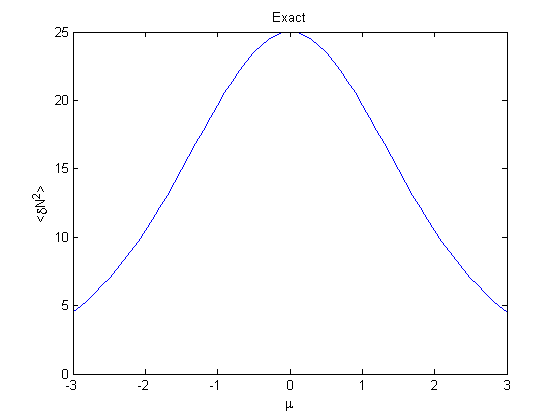
\includegraphics[scale=0.5]{prob1ii}
    \end{center}

  \item Our simulation values for $\langle (\delta N)^2 \rangle / M$ using $N_{step} = 10^4$ are shown below. For the bottom plot, my calculations for $\langle (\delta N)^2 \rangle / M$ ignore the $N$ values for the first 1000 iterations.
    \begin{center}
      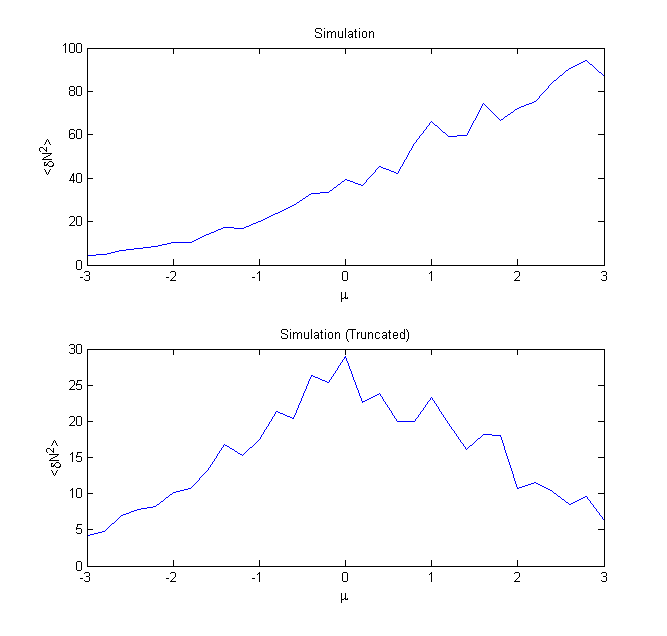
\includegraphics[scale=0.5]{prob1iii_10000}
    \end{center}

    Below are the results when I run the simulation with $N_{step} = 10^5$

    \begin{center}
      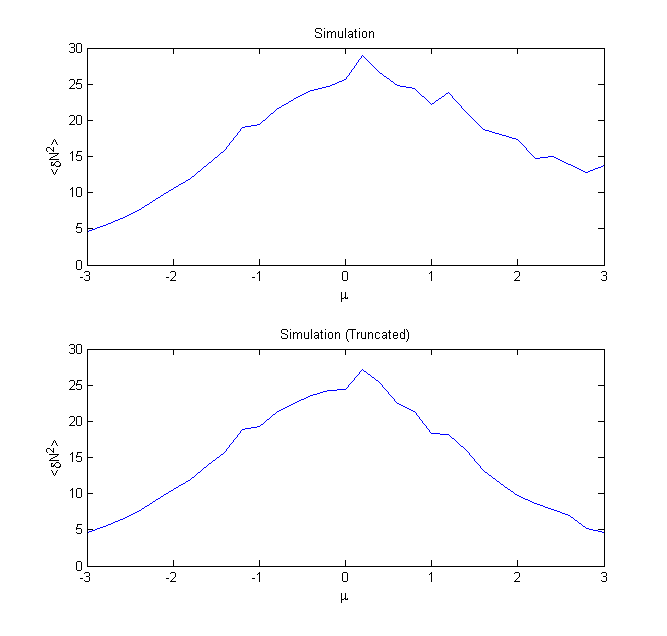
\includegraphics[scale=0.5]{prob1iii_100000}
    \end{center}

  \item The symmetry/accuracy of our numerical results highly depend on both the initial conditions and the sampling time. As I show in the plots for part (iii), we get much better results if we truncate off the values for the initial 1000 iteration of the simulation. This is because our system initially starts far away from the equilibrium state at $N=0$ particles, and as a result this skews are squared deviation values. Another way to offset the effect of the initial conditions is to run the simulation for a long period of time, thus makeing the initial skewed values a smaller proportion of the final result (as we see in the second graph in part(iii) where I run the simulation for an order of magnitude longer and arrive at fairly accurate results even without truncation).
\end{enumerate}


\section*{Problem 2}
\begin{enumerate}
  \item Let us define $N_1$ as the total number of particles in the config $v_1: (n_1,...,n_m)$ and $N_2$ as the number of particles in the config $v_2: (1-n_1,...,1-n_m)$. Let $M = N_1 + N_2$ be the total numer of lattice cells.
    \begin{center}
      \begin{align}    
        P(v_1) &\propto exp \left[\beta (\mu N_1 - E_1) \right] \\
        &= exp \left[\beta (-2\epsilon N_1 + \epsilon \sum\limits_{i, j} n_in_j) \right] \\
        P(v_2) &\propto exp \left[\beta (\mu N_2 - E_2) \right] \\
        &= exp \left[\beta (-2\epsilon (M-N_1) + \epsilon \sum\limits_{i, j} (1-n_in_j)) \right] \\
        &= exp \left[\beta (-2\epsilon (M-N_1) + \epsilon \sum\limits_{i, j} 1 - \epsilon\sum\limits_{i, j} n_in_j) \right] \\
        &= exp \left[\beta (-2\epsilon (M-N_1) + 2\epsilon M - \epsilon\sum\limits_{i, j} n_in_j) \right] \\
        &= exp \left[\beta (2\epsilon N_1 - \epsilon \sum\limits_{i, j} n_in_j) \right] \\
      \end{align}
    \end{center}

    Going from (9) to (10) we assume that every one of the $M$ cells has 4 neighbors (so neglecting ``edge'' cases). Thus the total number of unique pairwise interactions with closest neighbors is $2M$. I believe that my derivation is not correct because the final results (6) and (12) are not in agreement with one another; actually the expressions in the exponentials are opposites. The exponential function is not symmetric so from my results $P(v_1) \neq P(v_2)$...

  \item Using our MC simulation, the following plot is a histogram of our results for $P(N)$
    \begin{center}
      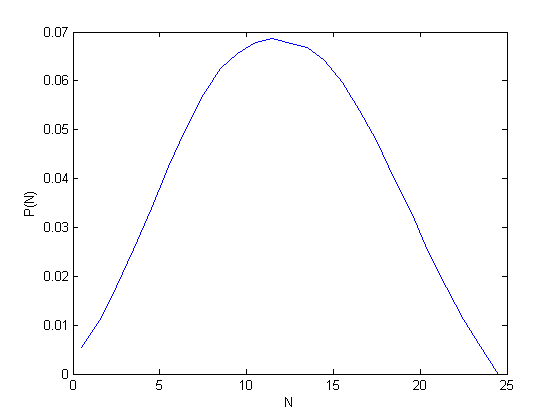
\includegraphics[scale=0.5]{prob2ii}
    \end{center}

  \item Below is a plot of our results for $P(N)$ for $T = 0.4,...,1.0$ using a lattice size of $M = 5 \times 5$
    \begin{center}
      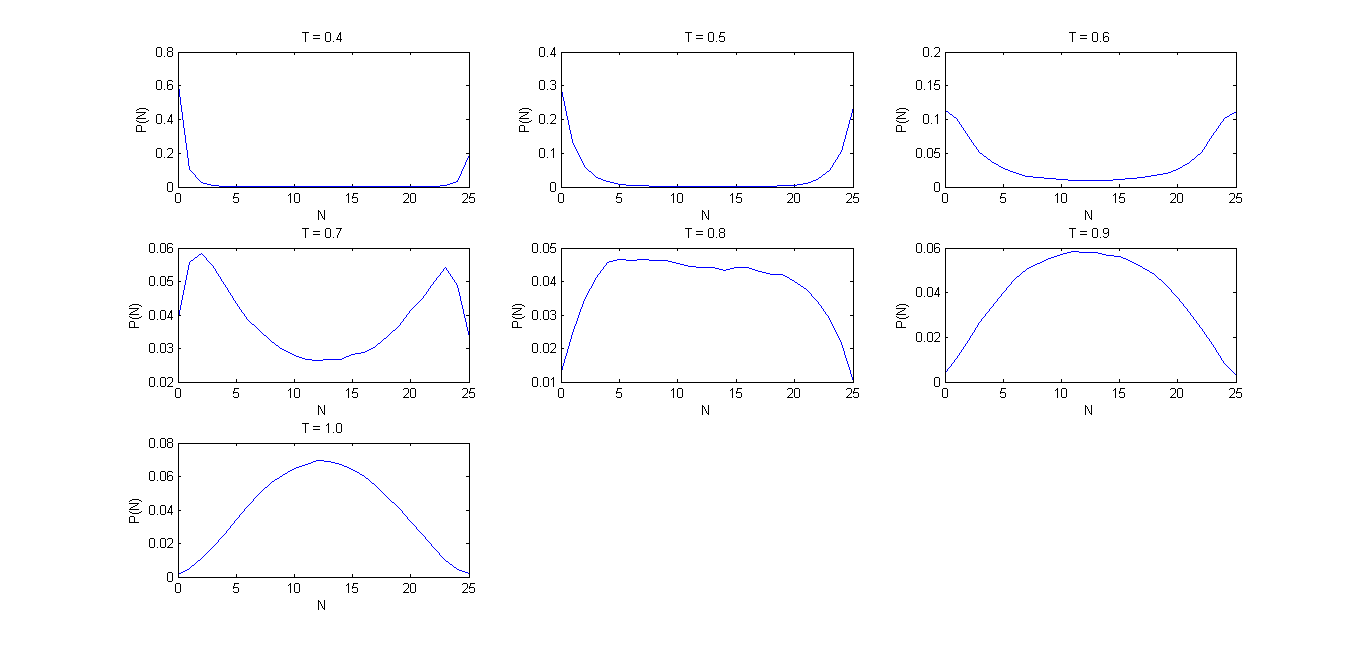
\includegraphics[scale=0.5]{prob2iii-1}
    \end{center}

    Additionally plots were also constructed for $M^-1 ln\left[P(N)/P(N*)\right]$
    \begin{center}
      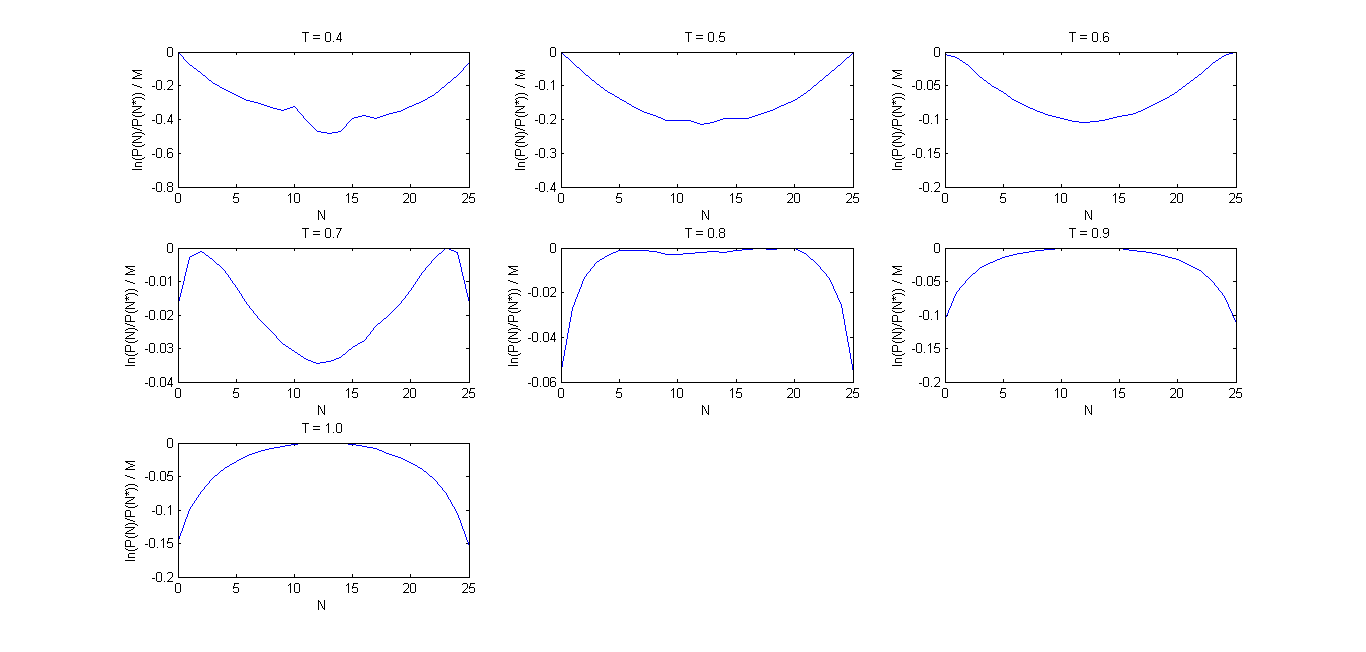
\includegraphics[scale=0.5]{prob2iii-2}
    \end{center}

  \item Below is a plot of my results for $P(N)$ for $T = 0.4,...,1.0$ using a lattice size of $M = 10 \times 10$
    \begin{center}
      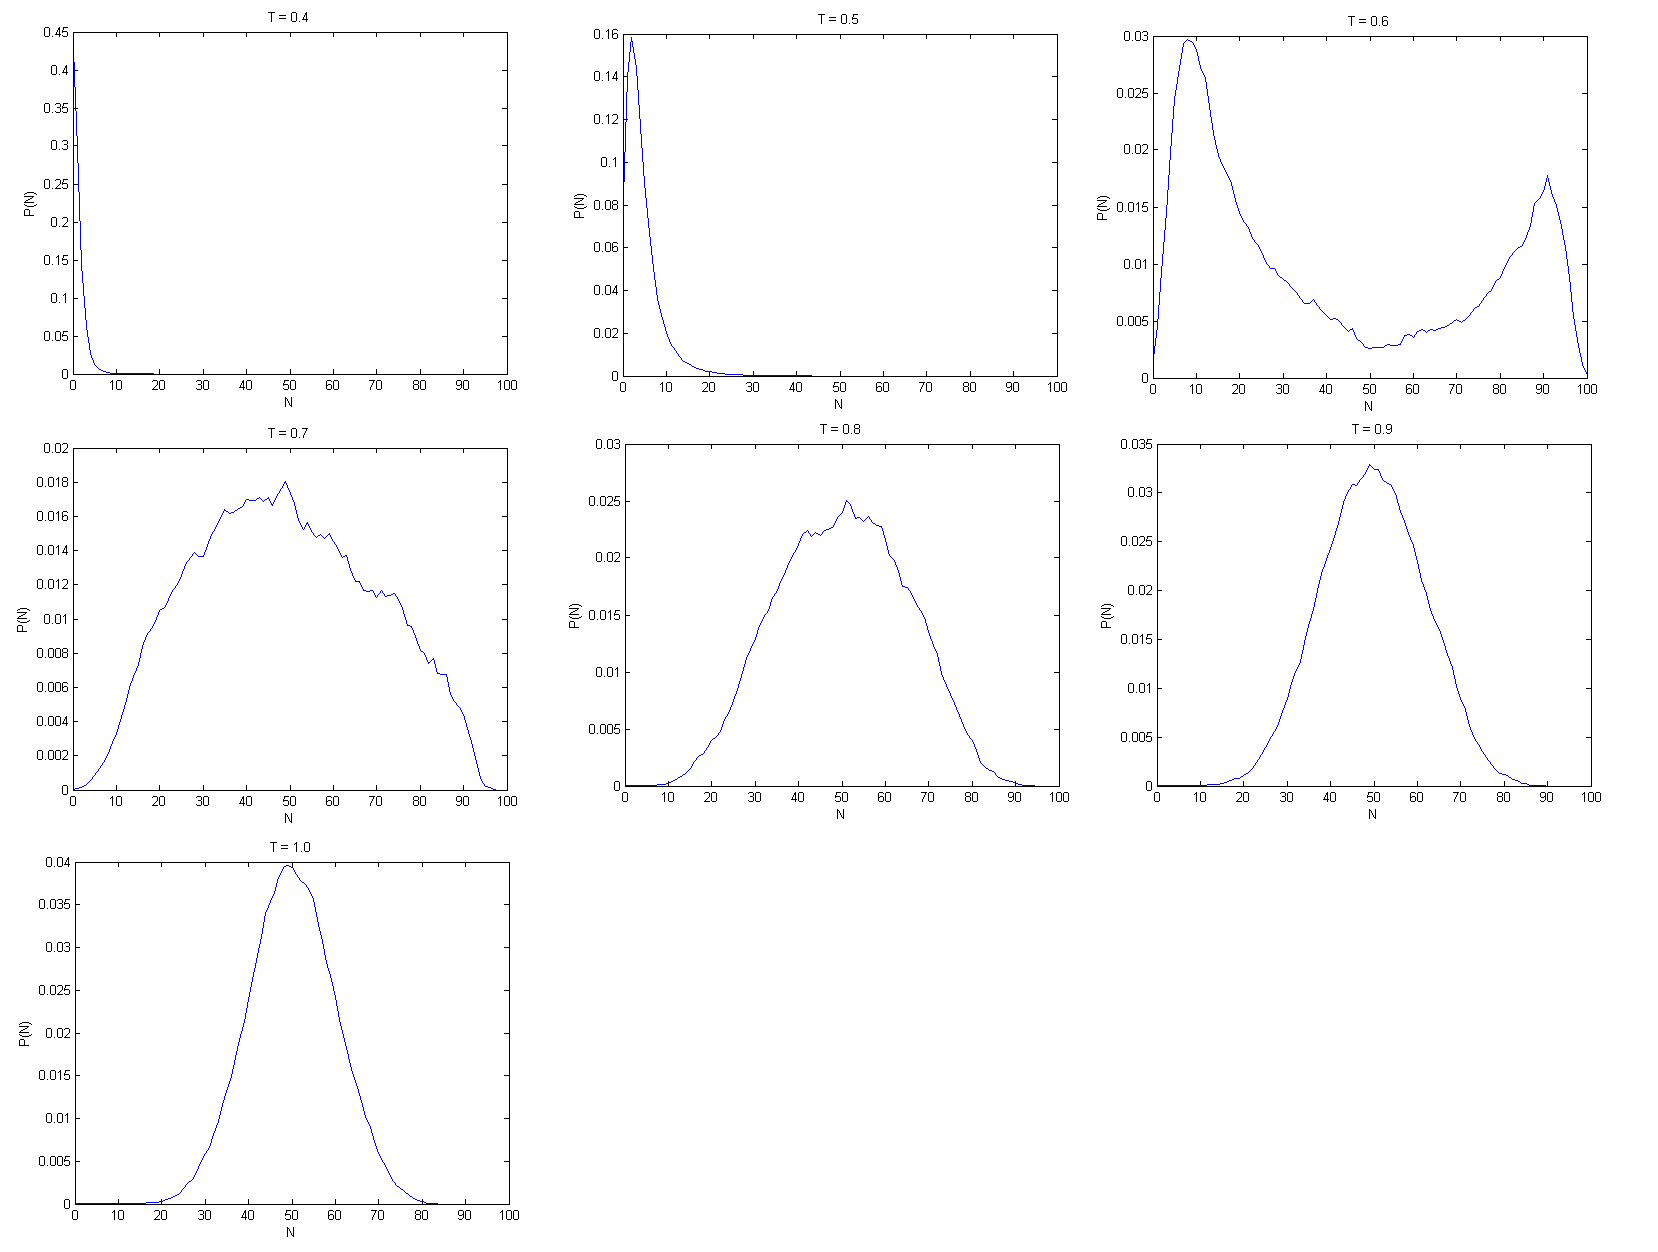
\includegraphics[scale=0.25]{prob2iv}
    \end{center}

    We note in particular that the lower temperature plots (particularly T=0.4,0.5) are unable to sample the second peak of the bimodal distribution. Recall the probability distributions should be bimodal/symmetric. This is because the lattice is initialized to have 0 occupancy and at low temperatures the probability of occupying any one cell is low. So if the lattice is too big and the temperature we're working with is relatively small, the probability of sampling larger $N$ (where $N$ is the total number of particles in the lattice) will be so small that it essentially won't happen unless the number of simulation steps is exhorbitantly large; the overall probability of observing $N$ is the product of the individual probabilities (which will be very small for low T) of observing cell i with $n_i$, multiplied by some combinatorial factor.

  \item In class we showed that if we want to swap to replicas:
    $$v : \{ x_a, T_1 ; x_b, T_2 \} \rightarrow v' : \{ x_b, T_1 ; x_a, T_2 \}$$

    Then the acceptance rule is as follows
    $$acc = min\left[ 1, e^{\Delta \beta \Delta E_{tot}}\right]$$

    In our case,
    \begin{center}
      \begin{align}    
        E_{tot} &= E(x_b) - E(x_a) \\
        &= (\mu N_b - E_b) - (\mu N_a - E_a) \\
        &= \mu (N_b - N_a) - (E_b - E_a) \\
        &= \mu \Delta N - \Delta E
      \end{align}
    \end{center}

    and,
    $$\Delta B = 1/T_2 - 1/T_1$$

  \item See \textit{latticegas\_parallel.m}

  \item Below is a plot of my parallel tempering results for $P(N)$ for $T = 0.4,...,1.0$ using a lattice size of $M = 10 \times 10$
    \begin{center}
      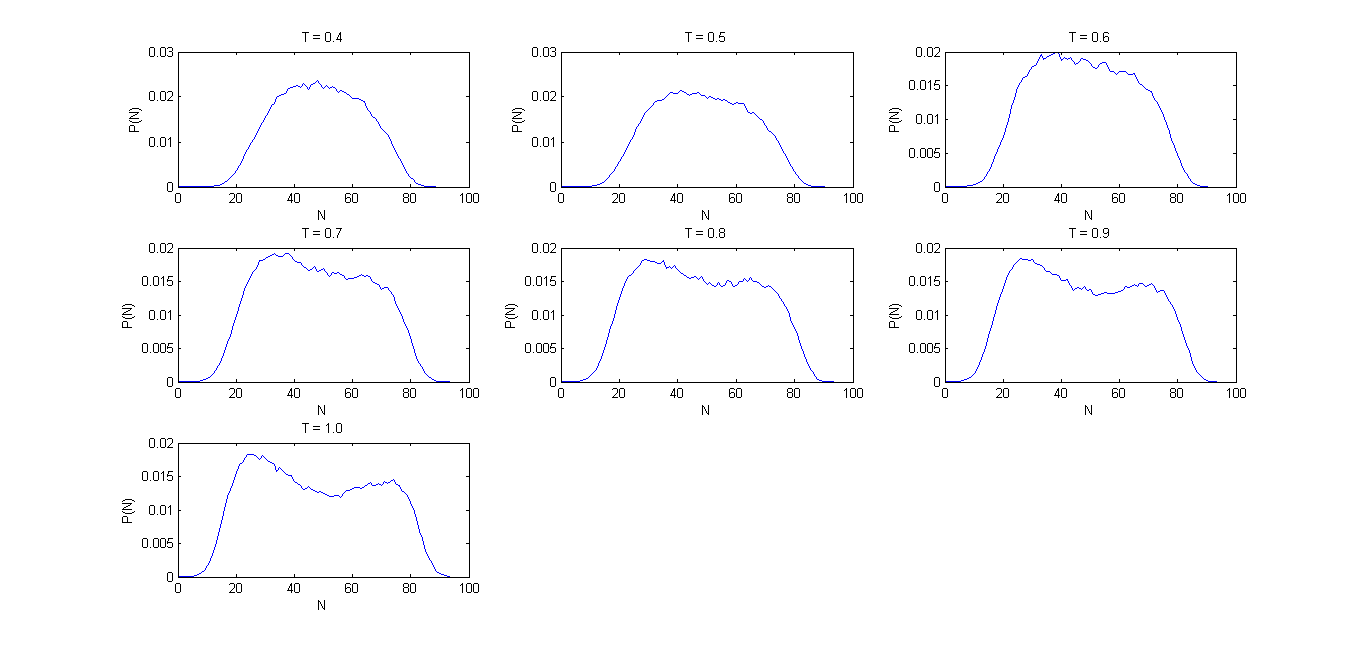
\includegraphics[scale=0.5]{prob2vii-1}
    \end{center}

    Actually I think that my plot indices are reversedand that the firstplot actually corresponds with $T=1.0$ and my last plot corresponds to $T=0.4$. I think I have an indexing bug somewhere but I don't have time to fix it... I will usse this assumption in my discussion below.

    We see that with parallel tempering, the low temperature states are now able to sample the bimodal distribution. This is the result of the occaisonal swapping of configurations, thereby allowing the low-T simulations to partake in the otherwise highly improbably (which is true physically but our simulation takes it to the extreme), more occupied states that the high-T simulations are more likely to sample. 

\end{enumerate}

\end{document}
